\documentclass[11pt,letter]{article}
\usepackage[top=1.00in, bottom=1.0in, left=1.1in, right=1.1in]{geometry}
\renewcommand{\baselinestretch}{1.1}
\usepackage{graphicx}
\usepackage{natbib}
\usepackage{amsmath}
\usepackage{textcomp}%amoung other things, it allows degrees C to be added
\usepackage{float}
\usepackage{hyperref}
\usepackage[utf8]{inputenc} % allow funny letters in citaions 
\usepackage[nottoc]{tocbibind} %should add Refences to the table of contents?
\usepackage{amsmath} % making nice equations 
\usepackage{graphicx} %including pictures 

\def\labelitemi{--}
\parindent=0pt

\title{Carl's Chardonnay Haridness Model \\ A guide on how it works }
\date{\today}
\author{Faith Jones}

\graphicspath{ {./Images/} }% tell latex where to find photos 

\begin{document}
%\renewcommand{\refname}{\CHead{}}%not sure what this was supposed to do 
\renewcommand{\bibname}{References}%names reference list 

\maketitle
\tableofcontents

\section{Introduction to the model}

Carl Bogdanoff is a viticulture researcher at AgCanada who has a particular interest in winegrape cold hardiness. He has been taking LTE$_{50}$ readings from various vineyards and varieties from 2012 to the present. With this data he has built models to track vine cold hardiness (in terms of LTE$_{50}$) in relation to air temperatures. With this model Carl is able to send growers predictions of how cold hardy their grapes are likely to be so the growers can better manage their activities. \\

A difficulty with the model is that it is coded in excel. This makes it difficulty to interact with the model. We would love to have work on this model but we need it in R. The first step with this model is therefore to get it working in R.\\

This document focuses on the Chardonnay model because this is the one Carl started with. There are other models for other varieties that are (maybe?) similar. \\ 

\section{Past work}
Faith coded up a previous version of the Chardonnay hardiness Carl sent us. Her code is in BCvin\textbackslash hardiness\textbackslash oldCarlModel\textbackslash. 

\begin{itemize} 
	\item hardiness\_stab.r. This is the main script Lizzie and Faith worked on to run Carl's older model. It used the functions below to replicate the if else statements in columns CC to CG. This file will be useful when setting up the data and as a reference for coding the full model. The files mentioned below will also be useful when trying to code if/else statements because you can see how they work, but I think the actual if/else statements will be quite different.     

	\item ColumnCC\_function.R
	\item ColumnCE\_function.R
	\item ColumnCF\_function.R
	\item ColumnCG\_function.R - this one does the rest of the columns. Because of the dynamic elements to these columns (the columns refer back to each other's values from the previous day) I had to make one giant loop.

	\item The old model is in BCvin\textbackslash hardiness\textbackslash fromCarl\textbackslash older.
\end{itemize}

\section{The new model}

\subsection{Overview of the model}
Carl's model works quite a bit differently from how we tend to write models in our lab, both structurally and mechanistically. The model's mechanics are spread out over various excel columns with functions coded into cells and columns are often repeated. Also the model has two main parts to it: estimating hardiness based on the day of the season and tweaking average hardiness each year to reflect the how the temperatures experienced that year deviate from average. These ``tweaks'' basically look at how much colder or warmer it is on the year of interest than the historical data, and increase or decrease vine hardiness accordingly. There are many if/else statements involved in these tweaks, and Carl likes to update them a little every year to ensure optimum fit.  

\subsection{The files}
\begin{itemize}
	\item Chard Model Instructions May 2020.docx. This is Carl's explanatory documents describing what he did and why. It is useful to refer to this document when coding the model in R. 
	\item Chard Model May 2020.xlsx. This is the actual model. Carl is an Excel wizard so all of the calculations happen here as well as any plotting and raw data. The file is fully explained in sections below.
\end{itemize}

\subsection{The data}

The model requires three data sets: 
\begin{enumerate}
	\item Hardiness measured in LTE$_{50}$ between 2012 and 2020. Various variety LTE${_50}$, including for Chardonnay, were measured at several sites in the Okenagan Valley by Carl and his team. Data was taken biweekly from late October to April. There was not a full season of data recorded for 2020 due to Covid-19. Each winter season is a separate csv file, and data are stored in analyses\textbackslash input\textbackslash budhardinessXtoY.csv, where X and Y are the years the data cover. These data can also be found in columns BB, BD, BF, BH, BJ, BL, BN and BP. There are lots of empty cells in these columns because we do not have LTE$_{50}$ data for most days nor the same day each year. 

	\item Mean 2 day temperature for between 2012 ans 2019, measured in \textdegree{}C, from Environment Canada's Penticton site. Stored in analyses\textbackslash input\textbackslash envcanada\_penticton.csv. These data are also in columns A though J of the spreadsheet. They are also repeated in columns R, U, X, AA, AD, AG, AJ and AM. 

	\item Historical temperature data which we pulled from Carl's excel file. Stored in analyses\textbackslash input\textbackslash climhist\_19812010.csv. These data are repeated many times in the spreadsheet so the mechanics of the model works. They first appear in column N (1981-2010 data: 2day), then they are repeated in columns CE, DB, DY onwards so they appear once for each year there is LTE$_{50}$ data.   

\end{enumerate}

\subsection{Preparing the data}
The model does uses mean 2 day temperature data, so that needs estimating. There is also code in hardiness\_stab.R that it estimates GDDs (Growing Degree Days) in case you need it. I do not think Carl's model uses GDDs though. 

\subsection{Estimating mean LTE$_{50}$ from day of the season}
This section of the model fits a 4$^{th}$ order polynomial curve to the LTE$_{50}$ values against day of the season. Carl uses the average LTE$_{50}$ values of Chardonnay, but we will want to use all the data instead so we can see how much variation there is between sites. This ``day of the season'' is the number of days since October 1$^{st}$, which is the beginning of winter hardiness acclimation according to Carl (Figure \ref{fig:LTEperDay}). The purpose of this section is to get a ``general'' trend of how LTE$_{50}$ changes throughout the dormant season. The columns where this takes place are BR to BZ. Note the previous model Carl sent that we coded up uses a very different approach to getting the average trend of LTE$_{50}$ so there will be big chunks of hardiness\_stab.R that are not relevant to the new model. I think the equation is:
\begin{equation*}
PredLTE_{50} = 12.29*cd^{4} - 42*cd^{3} + 63*cd^{2} - 44*cd - 13
\end{equation*}
where $PredLTE_{50}$ is the predicted hardiness that day (day since October 1$^{st}$), and $cd$ is the day since October 1$^{st}$/100. $PredLTE_{50}$  is in column BY and $cd$ is in column BX. \\
  
\begin{figure}[H]
  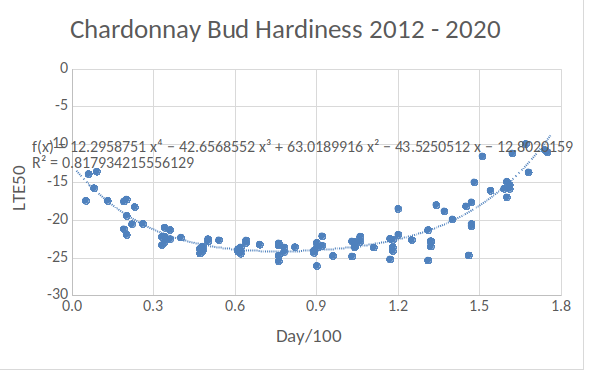
\includegraphics[width=\linewidth]{FiguredLTEday.png}
  \caption{A plot taken from Carl's May 2020 Chardonnay excel model (Chard Model May 2020.xlsx). A polynomial 4$^{th}$ order curve is used to estimate LTE$_{50}$ each day of the hardiness season.}
  \label{fig:LTEperDay}
\end{figure}

The estimated LTE$_{50}$ values are repeated  for 2012/2013 in column CG (Estimate LTE), and the change between days is in column CG (Estimate LTE/day). They are also repeated are also repeated further to the right in the spreadsheet for every other year. 

\subsection{Tweaking hardiness or the year of interest}

Once you have estimated LTE$_{50}$ values for each day of the season then you can get predicted LTE$_{50}$ values for a day of the season based on air temperatures that season. \\

The first step in this process is using the historical data as a baseline, and seeing how much colder it is on the day and year of interest than this historical value. These calculations happen in columns Q t AO. If the 2 day mean temperature for your day of interest (for example 28$^{th}$ Sep 2015) is 10.7 \textdegree{}C, and the average temperature for the 28$^{th}$ Sep in the historical data is 12.3 \textdegree{}C, then the difference is -1.6 \textdegree{}C. That is, in 2015 this day was a fair bit colder than the average for that day. This cell will be coloured blue on the spreadsheet, and warmer values will be coloured red. The basic idea is that the cold hardiness of a vine on the 28$^{th}$ of September 2015 will be colder than the average LTE$_{50}$ predicted by the polynomial curve. Exactly how much colder is the next step of the model. The difference between historical temperatures and the day and year of interest is repeated later in the spreadsheet. For example, the difference between historical and 2012/2013 data is in column CH. \\

Carl estimates LTE$_{50}$ each season separately. I will walk you through the 2012/13 data (see Figure \ref{fig:201213Calculation}). You will hopefully already be familiar with some of these columns from teh sections above, but I will repeat what each one contains to avoid confusion.
\begin{itemize}
	\item CC: day of the year. Carl starts estimating hardiness from the 20$^{th}$ of September, but had temperature data before that and for some reason lists dates from September 1$^{st}$). 
	\item CD-CE: Historic temperatures. You only need concern yourself with the 2 day average (column CE). 
	\item CF: Estimated LTE$_{50}$. Values are taken from the polynomial curve mentioned above. 
	\item CG: Estimated LTE/day. This is how different each LTE$_{50}$ value is from the value the previous day, so it is the rate of change of LTE$_{50}$ per day. Values can increase or decrease. 
	\item CH: A repeat of column S. This is difference between the temperature that day and the historical mean for that year. 
	\item CI-CV: A selection of if/else statements that change the estimated LTE$_{50}$ based on the polynomial curve to a specific estimated LTE$_{50}$ for that specific date. Note that the statements change within a column, for example the statement in the autumn might be different from midwinter. Some of the later columns depend on each other a lot more so will need to be coded as one big function rather than a single function for each column. For more details on the statements in these columns see Chard Model Instructions May 2020.docx, and for how we previously tackled these type of columns see hardiness\_stab.R. 
	\item CW: Final predicted LTE$_{50}$ values for that season based on temperatures that year.
\end{itemize}

\begin{figure}[H]
  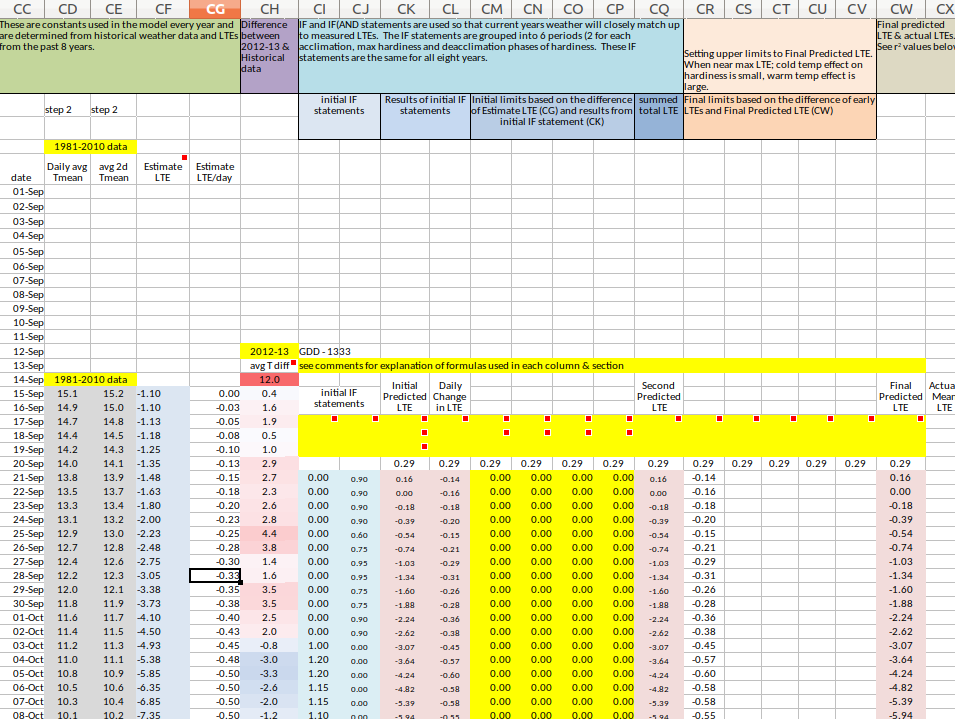
\includegraphics[width=\linewidth]{201213Calculation.png}
  \caption{A screen shot of the section of Carl's model spreadsheet  (Chard Model May 2020.xlsx) where the tweaks for each year are calculated. This example is 2012/2013, and the same layout is repeated in columns to the right for the rest of the years.}
  \label{fig:201213Calculation}
\end{figure}

\bibliographystyle{/home/faith/Documents/Bibtex/styles/besjournals/besjournals}
\bibliography{/home/faith/Documents/Bibtex/mendeleyStuff/library}

\end{document}



